\section{R\"uckblick} 
\frame{\frametitle{Konzept der LRP}
\begin{itemize}
\item Gem\"ass bestimmter Formeln soll die Relevanz einzelner Pixel durch eine "{}R\"uckrechnung"{} aus dem Output visualisiert werden. 
\item Einfachste Form: 
\begin{align}
R_{i}^{(l)}=\sum_{j} \frac{z_{i j}}{\sum_{i^{\prime}} z_{i^{\prime} j}} R_{j}^{(l+1)} \quad \text { mit } \quad \mathrm{z}_{\mathrm{ij}}=\mathrm{x}_{\mathrm{i}}^{(1)} \mathrm{w}_{\mathrm{ij}}^{(1,1+1)}
\end{align}
\item Am Beispiel des MNIST Datensatz:
\end{itemize}
\begin{figure}
\centering
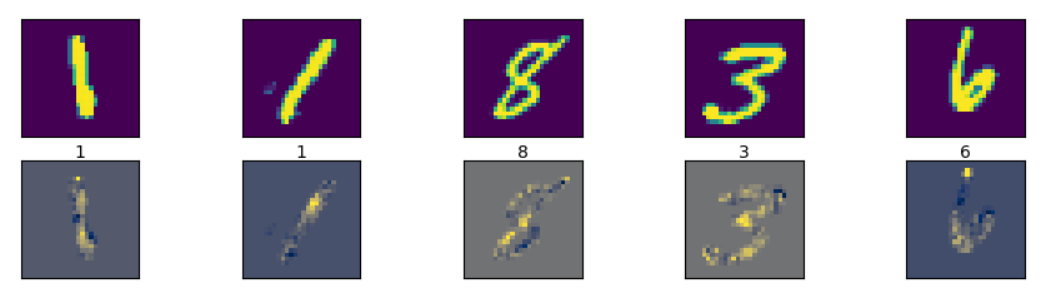
\includegraphics[width=0.6\textwidth]{grafiken/mnist_erg_1.png}
\end{figure}
}


\frame{\frametitle{Vergleich LRP $\leftrightarrow$ Heatmap}
\begin{itemize}
\item Ersetze den Wert der Neuronen $x_i$ durch den Mittelwert der Schicht.
\item Versuche, allgemeine Aussagen zu treffen.
\item Am Beispiel des MNIST Datensatz:
\item <Screenshot machen und hinzu>
\end{itemize}
%\vspace*{1cm}


}
